\chapter*{Introducción}\label{cha:introduccion}
\addcontentsline{toc}{chapter}{Introducción}
\markboth{Introducción}{Introducción}

\AddToShipoutPictureBG*{\put(0,0){%
    \parbox[b][\paperheight]{\paperwidth}{%
      \vfill
      \centering
      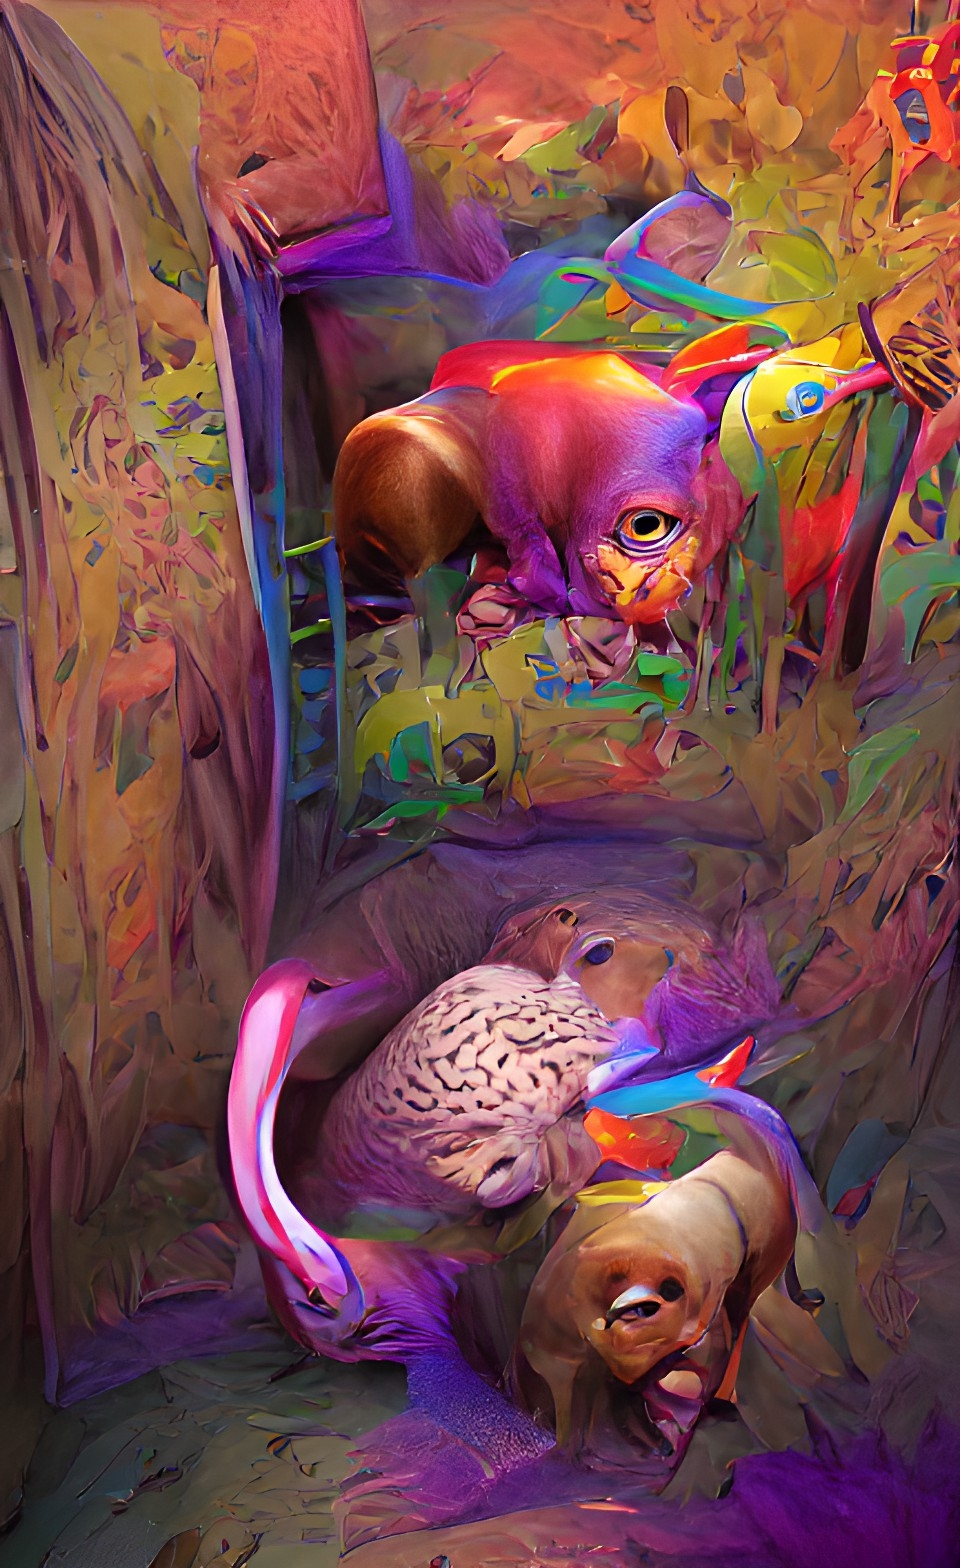
\includegraphics[width=\paperwidth,height=\paperheight,keepaspectratio]{%
        figuras/caratulas/analisis_no_supervisado_del_comportamiento_animal.jpg}\vfill
    }}}

\AddToShipoutPicture*{
  \begin{tikzpicture}[overlay, remember picture]
    \fill[white, opacity=0.75] (20, 24) rectangle (1, 22.5);
  \end{tikzpicture}}

\clearpage

En la última década, ha empezado a consolidarse un nuevo campo en la neurociencia del comportamiento: la etología computacional. Esta consiste en el uso de herramientas de visión artificial y técnicas de aprendizaje automático para medir y analizar patrones de comportamiento animal con mayor grado de detalle en entornos cada vez más complejos, similares a los naturales y ecológicamente relevantes (esto es, relativos a la supervivencia de la especie y a la adaptabilidad al entorno). El avance en la investigación en este campo ha sido posible gracias al progreso técnico en inferencia estadística y en redes neuronales artificiales, a la democratización del acceso a computadoras de alto rendimiento (tanto por la reducción de costos de \textit{hardware} y por la popularización de servicios de \textit{cloud computing}) y por la aplicación de nuevas tecnologías en la resolución de problemas de la biología computacional \cite{datta_computational_neuroethology}.

En el campo de la neurociencia, el enfoque de la etología computacional es no solo prometedor sino necesario para acompañar el progreso tecnológico en el registro de la actividad neuronal \textit{in vivo}. En un futuro donde se tenga acceso a registros de cientos de miles de neuronas, estos podrán estudiarse con relación a comportamientos animales más complejos, caracterizados por miles de variables dinámicas y descritos en mayor detalle. De esta manera, esperamos que el análisis de patrones neuronales de alta dimensionalidad se vea beneficiado, o incluso facilitado, por el uso de descripciones comportamentales cuya complejidad y dimensionalidad sea más cercana a la del espacio de registros neuronales estudiado (\autoref{fig:introduccion_registros_neuronas}) \cite{datta_computational_neuroethology, glaser_kording_multimodal_neuroscience, neuron_recording_duplication, lecoq_neuron_microscopy, demas_lbm, chen_neuron_recording_scales}.

\begin{figure}[htbp]
  \centering
  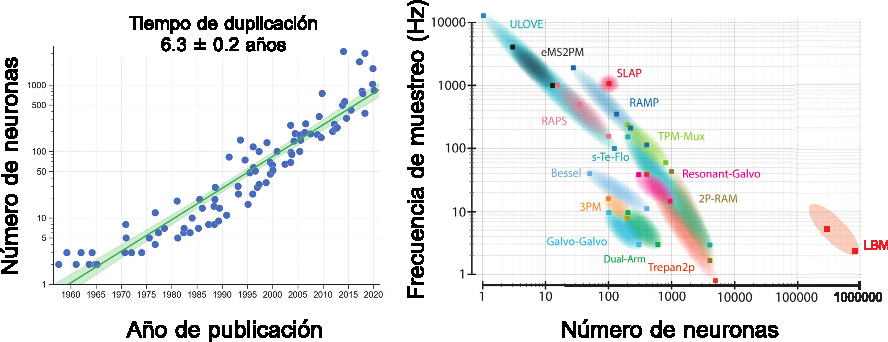
\includegraphics[width=0.99\linewidth]{figuras/introduccion/registros_neuronas.pdf}
  \caption{\textbf{Número de neuronas registradas se duplica cada 6 años.} (Izquierda) Aumento del número de neuronas registradas usando arreglos multielectrodos en estudios publicados entre los años 1957 y 2020. (Derecha) Relación entre la frecuencia de muestreo y el número de neuronas registradas usando métodos de microscopía. Las técnicas más recientes (LBM) registran un millón de neuronas a una frecuencia de muestreo de 2 Hz \cite{neuron_recording_duplication, lecoq_neuron_microscopy, demas_lbm, chen_neuron_recording_scales}.}
  \label{fig:introduccion_registros_neuronas}
\end{figure}

Desde esta perspectiva se hace un llamado al desarrollo de métodos que combinen el análisis del comportamiento animal en entornos naturales con los patrones de actividad neuronal y los circuitos involucrados. La neuroetología computacional avanza en este sentido: investigar las relaciones entre el comportamiento animal complejo y los registros neuronales para entender mejor el funcionamiento del cerebro.

En este trabajo, exploramos aplicaciones de la estadística y del aprendizaje automático para el análisis del comportamiento animal. Sin embargo, un problema común en la manipulación de grandes volúmenes de datos de alta dimensionalidad es la difícil interpretabilidad de los datos y modelos utilizados para estudiarlos. Por ejemplo, los modelos de aprendizaje automático basados en redes neuronales profundas pueden generar predicciones muy precisas para una amplia gama de problemas; sin embargo, suele ser difícil de interpretar su funcionamiento interno y esclarecer los mecanismos de inferencia del modelo \cite{molnar_interpretable_machine_learning}.

Aquí es donde entran en juego los mapas no lineales, para la visualización y reducción de la dimensión de conjuntos de datos. Estos mapas son una herramienta popularizada recientemente en diversos ámbitos, desde el análisis de secuenciamiento de células individuales en bioinformática, pasando por el estudio de similaridad de textos en el análisis de lenguaje natural, hasta sistemas de recomendación de productos usados en la industria de la información \cite{packer_umap_c_elegans, mikolov_word2vec, recommendation_systems}. Incluso se utilizan para interpretar el funcionamiento de redes neuronales artificiales profundas \cite{carter_activation_atlas}.

En este aspecto, la etología computacional no es una excepción. Especialmente considerando que abundan los registros de video de comportamiento animal, gracias al fácil acceso a cámaras digitales y su versatilidad para ser incorporadas en la mayoría de los protocolos experimentales existentes. En simultáneo, la aparición de herramientas de \textit{software} para la captura de movimiento sin marcadores físicos, abrieron la puerta a una cantidad impensada de datos crudos. En este contexto de abundancia de datos y de registros comportamentales cuantitativos, cada vez más detallados y de mayor dimensionalidad, son cada vez más útiles los mapas no lineales para reducción de la dimensión \cite{berman_mapping}.

Pero, para que un mapa de dimensión reducida tenga sentido como representación de un conjunto de datos de mayor dimensionalidad, deben satisfacerse algunas condiciones. Principalmente, el conjunto de datos en cuestión debe tener una estructura interna de dimensionalidad baja y debemos tener acceso a una muestra representativa de esta estructura (\textit{manifold hypothesis}) \cite{manifold_hypothesis}. Afortunadamente, en etología, se trabaja bajo el supuesto de estereotipia. Este consiste en que los comportamientos exhibidos por un animal pueden ser descompuestos en elementos discretos y reproducibles, y, por lo tanto, pueden representarse en un espacio de dimensión baja. Estos comportamientos elementales se suponen constantes a lo largo del tiempo y consistentes entre diferentes individuos y, en algunos casos, entre diferentes especies \cite{hernandez_fly_species}. Estos conjuntos discretos de comportamientos podrían emerger a partir de diferentes mecanismos, por ejemplo, la existencia de restricciones biomecánicas para el control de la locomoción animal, la aparición y conformación de hábitos, o la presión selectiva para ejecutar acciones robustas u óptimas en un determinado entorno natural. Estos mecanismos limitan el repertorio de movimientos de los animales, a pesar de su potencial capacidad de moverse de infinitas maneras en un espacio continuo, restringidos en principio únicamente por los límites biomecánicos de su morfología \cite{berman_mapping, lehner_stereotipy}.

El concepto de estereotipia tiene una gran utilidad cuando se trata de comprender cómo el cerebro controla dichas acciones.
En este caso, la información resultante de la cuantificación del comportamiento es de fundamental importancia para su correlación con registros simultáneos de la actividad neuronal con el fin de estudiar cómo el cerebro codifica diferentes comportamientos, cuáles son los circuitos neuronales subyacentes y cómo estos se modifican durante el aprendizaje de nuevas tareas motoras \cite{esposito_defensive, levy_representation}. A pesar de su importancia, la determinación del repertorio de comportamientos de un animal resulta experimentalmente complicada, debido a las dificultades que conlleva la cuantificación del comportamiento animal en términos objetivos, reproducibles y utilizando sistemas automatizados. Afortunadamente, en los últimos años se popularizaron métodos de análisis no supervisado del comportamiento, utilizando algoritmos de reducción de la dimensión. En la literatura existen ejemplos de aplicación de estos métodos de análisis del comportamiento animal en gusanos, moscas, peces cebra y ratones, durante el desarrollo de tareas de \textit{open field} \cite{stephens_eigenworms, zebrafish_unsupervised, berman_mapping, berman_hierarchy, markowitz_mouse_behavior, mouse_autism_open_field}.

\clearpage

En este trabajo, estudiamos el espacio de comportamientos a los que accede un conjunto de 10 ratones realizando una tarea de aprendizaje motor. La tarea estudiada se denomina rotarod con aceleración, y consiste en entrenar ratones para que caminen sobre un cilindro que gira a velocidades crecientes, con aceleración constante en su rotación. El rotarod con aceleración es un paradigma experimental ampliamente utilizado en el estudio del aprendizaje motor dado que el rendimiento del animal mejora con el entrenamiento de manera dependiente de la plasticidad neuronal \cite{costa_motor_learning, mouse_tests}. Originalmente, al aparato rotarod fue diseñado para evaluar déficit neurológico e impedimento motor en roedores, y es actualmente uno de los métodos más comunes para medir rendimiento y aprendizaje motor \cite{dunham_rotarod, mouse_tests}. Sin embargo, el desempeño del animal en esta tarea se suele evaluar simplemente a través de la medición del tiempo de permanencia sobre el cilindro (latencia a caer). Bajo esta situación nos preguntamos, ¿cuáles son los cambios en el repertorio de movimientos de un animal asociados a un mejor desempeño de la tarea?, ¿existen diferencias entre los individuos respecto de las estrategias que utilizan para resolver la tarea?

Para responder estas preguntas, realizamos una serie de filmaciones de los animales mientras realizaban la tarea, usando un arreglo de 2 cámaras digitales. Para cuantificar sus movimientos, se extrajeron coordenadas bidimensionales de las posiciones de algunas partes de sus cuerpos y su evolución en el tiempo. Para ello, se utilizó DeepLabCut, un \textit{software} de captura de movimiento de código abierto, que no requiere la utilización de marcadores físicos adicionales sobre los cuerpos de los animales \cite{mathis_deeplabcut}. A partir de estas coordenadas se calcularon posiciones relativas en función del tiempo. De esta manera, se extrajo información cuantitativa de las posiciones de los ratones y de sus partes del cuerpo durante el transcurso de cada prueba realizada en el rotarod.

Primeramente, propusimos métricas de rendimiento, alternativas a la latencia a caer del ratón, para mostrar los diferentes grados de aptitud física y de aprendizaje de la tarea entre individuos. Estas métricas ilustran una manera multidimensional de representar el comportamiento animal a lo largo de una prueba rotarod. El próximo paso es encontrar representaciones del comportamiento de menor dimensionalidad.

Para ello, usamos el algoritmo UMAP de aprendizaje automático no supervisado. Este algoritmo se utilizó para construir mapas no lineales y producir dos posibles representaciones del comportamiento de los ratones, en un espacio latente de dimensión baja \cite{mcinnes_umap}. El algoritmo UMAP es también una herramienta popular para la visualización de conjuntos de datos de dimensión alta y se utiliza frecuentemente en el ámbito de la bioinformática para visualizar datos provenientes de la secuenciación del material genético de células individuales \cite{packer_umap_c_elegans}.

Uno de los mapas UMAP fue construido usando los espectros de frecuencia \textit{wavelet} de las partes del cuerpo de los ratones. Los espectros \textit{wavelet} capturan información sobre la dinámica del movimiento de los ratones a diferentes escalas temporales en varios canales de frecuencia. En particular, estos espectros son especialmente sensibles a la ocurrencia de intervalos de movimiento periódico \cite{berman_mapping}.

El otro mapa UMAP fue construido usando características extraídas de los pasos y poses ejecutadas por los ratones durante la prueba. Estas características tienen escalas de variación temporal más cortas que los espectros \textit{wavelet} y conservan información sobre la posición de los ratones en el tiempo y el desfasaje entre sus partes del cuerpo.

\clearpage

\begin{figure}[htbp]
  \centering
  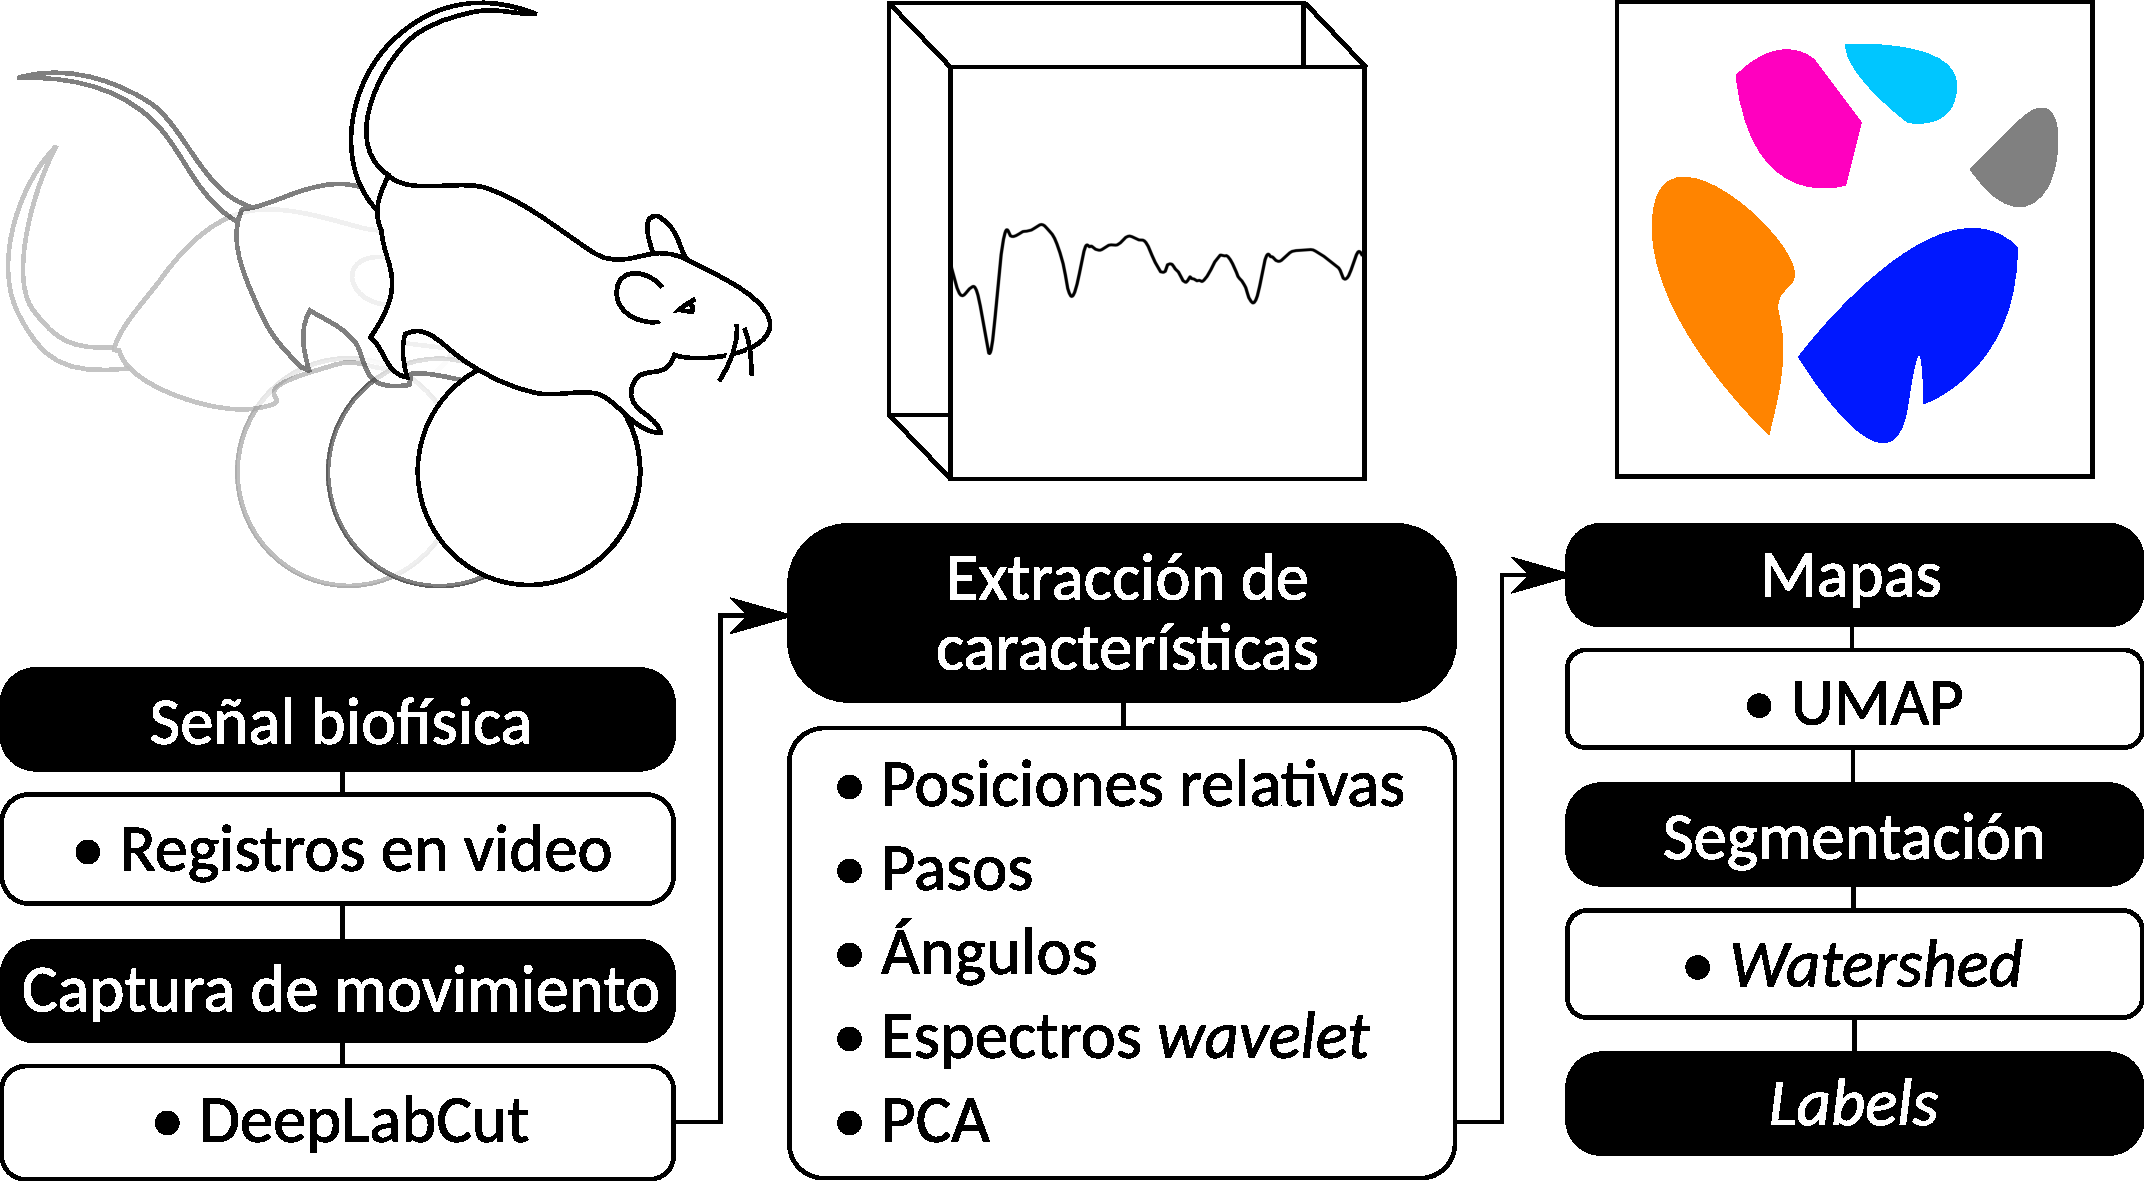
\includegraphics[width=0.85\linewidth]{figuras/introduccion/flujo_de_trabajo.pdf}
  \caption{\textbf{Obtención de mapas de comportamiento.} Esquema simplificado del flujo de trabajo utilizado para obtener mapas comportamentales.}
  \label{fig:introduccion_flujo_de_trabajo}
\end{figure}

Finalmente, se agruparon los comportamientos observados en categorías (\textit{labels} de comportamiento), realizando segmentaciones \textit{watershed} sobre los mapas, y se caracterizaron estos comportamientos (\autoref{fig:introduccion_flujo_de_trabajo}). De esta manera, dilucidamos la estructura subyacente y la dinámica del comportamiento, mejorando nuestro entendimiento acerca de la ejecución y el aprendizaje de esta tarea. Los comportamientos encontrados separan a los ratones en grupos de rendimiento, y la manera en que estos comportamientos son utilizados se consolida durante el entrenamiento. En particular, algunos comportamientos son utilizados exclusivamente por ratones de rendimiento alto o de rendimiento bajo. Además, la variabilidad con la que se utilizan algunas estrategias comportamentales se reduce con el entrenamiento.